\chapter{Análisis del problema}
 
En todo proceso de Ingeniería del \textit{Software} se necesita seguir un procedimiento muy
metódico y preciso, dividiendo el desarrollo del \textit{software} en distintas fases que
nos ayudarán a conseguir un producto que se ajuste a las necesidades que requiere el
problema.

\section{Ingeniería de requisitos}
Durante esta fase se cubrirán y proporcionarán las técnicas y los mecanismos apropiados
para:

    \begin{itemize}
        \item Analizar y entender las necesidades de los arqueólogos.
        \item Evaluar la viabilidad de las distintas propuestas (necesidades).
        \item Negociar una solución razonable/viable para ambas partes.
        \item Controlar y administrar los requisitos a lo largo del proceso de desarrollo.
    \end{itemize}

\subsection{Requisitos funcionales}
Describen la interacción entre la Aplicación Web y su entorno (base de datos, usuarios, 
comunicación con la App Android, etc.), indicando cómo debe actuar frente a situaciones o
entradas determinadas.

    \begin{itemize}
        \item \textbf{RF-1}. Gestión de excavaciones.
            \begin{itemize}
                \item \textbf{RF-1.1}. Consultar excavación.
                \item \textbf{RF-1.2}. Añadir excavación.
                \item \textbf{RF-1.3}. Modificar excavación.
                \item \textbf{RF-1.4}. Eliminar excavación.       
                \item \textbf{RF-1.5}. Descargar informe.       
                \item \textbf{RF-1.6}. Consultar unidades estratigráficas asociadas.            
            \end{itemize}
        \item \textbf{RF-2}. Gestión de estancias.
            \begin{itemize}
                \item \textbf{RF-2.1}. Consultar estancia.
                \item \textbf{RF-2.2}. Añadir estancia.
                \item \textbf{RF-2.3}. Modificar estancia.
                \item \textbf{RF-2.4}. Eliminar estancia.       
            \end{itemize}
        \item \textbf{RF-3}. Gestión de hechos.
            \begin{itemize}
                \item \textbf{RF-3.1}. Consultar hecho.
                \item \textbf{RF-3.2}. Añadir hecho.
                \item \textbf{RF-3.3}. Modificar hecho.
                \item \textbf{RF-3.4}. Eliminar hecho. 
                \item \textbf{RF-3.5}. Consultar unidades estratigráficas asociadas.          
            \end{itemize}
        \item \textbf{RF-4}. Gestión de unidades estratigráficas.
            \begin{itemize}
                \item \textbf{RF-4.1}. Consultar unidad estratigráfica.
                \item \textbf{RF-4.2}. Añadir unidad estratigráfica.
                \item \textbf{RF-4.3}. Modificar unidad estratigráfica.
                \item \textbf{RF-4.4}. Eliminar unidad estratigráfica.          
            \end{itemize}
        \item \textbf{RF-5}. Gestión de inventario fotográfico.
            \begin{itemize}
                \item \textbf{RF-5.1}. Consultar fotografía.
                \item \textbf{RF-5.2}. Añadir fotografía.
                \item \textbf{RF-5.3}. Modificar fotografía.
                \item \textbf{RF-5.4}. Eliminar fotografía.    
            \end{itemize}
        \item \textbf{RF-6}. Gestión de materiales.
            \begin{itemize}
                \item \textbf{RF-6.1}. Consultar material.
                \item \textbf{RF-6.2}. Añadir material.
                \item \textbf{RF-6.3}. Eliminar material.    
            \end{itemize}
        \item \textbf{RF-7}. Gestión de usuarios.
            \begin{itemize}
                \item \textbf{RF-7.1}. Registrar usuario.
                \item \textbf{RF-7.2}. Activar usuario (arqueólogo administrador).
                \item \textbf{RF-7.3}. Modificar contraseña.
                \item \textbf{RF-7.4}. Recuperar de contraseña.
                \item \textbf{RF-7.5}. Desactivar usuario.
                \item \textbf{RF-7.6}. Cambiar grupo.
            \end{itemize}
    \end{itemize}

\subsection{Requisitos no funcionales}
Este tipo de requisitos describen restricciones o cualidades de nuestra aplicación web que
no tienen una relación directa con las funcionalidades del sistema.

    \begin{table}[H]
        \centering
        \begin{tabular}{|l |l |} \hline

            \textbf{RNF-1} 
             & \underline{Eficiencia} \\
             & \tabitem El sistema tiene que tener un tiempo de respuesta corto.  \\
             & \tabitem El sistema tiene que ser capaz de almacenar gran cantidad de \\
             & excavaciones. \\ \hline

             \textbf{RNF-2} 
             & \underline{Usabilidad} \\
             & \tabitem Tiene que ser compatible con ordenadores, móviles y tabletas.  \\
             & \tabitem Fácil de usar, se hará un uso intuitivo de forma sencilla. \\ \hline

             \textbf{RNF-3} 
             & \underline{Seguridad} \\
             & \tabitem Acceso al sistema con usuario y contraseña únicos.  \\
             & \tabitem Cada usuario verá únicamente su información privada. \\ \hline

             \textbf{RNF-4} 
             & \underline{Legalidad} \\
             & \tabitem Debe cumplir la legislación sobre la gestión de información. \\
             & confidencial \\ \hline

             \textbf{RNF-5} 
             & \underline{Disponibilidad} \\
             & \tabitem El sistema debe estar disponible el máximo tiempo posible. \\ \hline

             \textbf{RNF-6} 
             & \underline{Implementación} \\
             & \tabitem Debe ser accesible desde un dispositivo móvil.  \\
             & \tabitem Debe ser accesible desde un navegador web. \\ \hline

             \textbf{RNF-7} 
             & \underline{Operaciones} \\
             & \tabitem Si se requiriese alguna modificación, esta la realizará el \\
             & administrador.  \\ \hline

             \textbf{RNF-8} 
             & \underline{Soporte} \\
             & \tabitem Durante el mantenimiento, el sistema estará inoperativo. \\ \hline

        \end{tabular}
        \caption{Tabla de requisitos no funcionales}
        \label{tab:rfn-table}
    \end{table}


\subsection{Requisitos de información}
Este tipo de requisitos describirán necesidades de almacenamiento de información en
la aplicación web.

\begin{table}[H]
    \centering
    \begin{tabular}{|l |l |} \hline

        \textbf{RI-1} 
         & \underline{Usuarios} \\
         & \tabitem Información necesaria de los usuarios a la hora de registrarse en la \\
         & aplicación.  \\
         & \tabitem \textbf{Contenido}: nombre, correo electrónico, contraseña. \\ 
         & \textbf{Requisitos asociados}: RF-7 \\ \hline

    \end{tabular}
    \caption{Tabla de requisitos de información}
    \label{tab:ri-table}
\end{table}

\section{Descripción de actores} \label{sec:actors}
\subsection{Usuario no registrado}
    \begin{table}[H]
    \begin{center}
        \begin{adjustbox}{width=\textwidth}
        \begin{tabular}{ | l | l | l | l | c | c | } 
            \hline
            \textbf{Actor} & \multicolumn{4}{l|}{Usuario no registrado} & \cellcolor{gray!50} \textbf{ACT-1}\\
            \hline
            \textbf{Descripción} & \multicolumn{5}{p{0.9\linewidth}|}{Representa a un usuario
            que accede por primera vez al sitio y aún no ha enviado la petición de registro.} \\
            \hline
            \textbf{Características} & \multicolumn{5}{p{0.5\linewidth}|}{No está registrado
            en el sistema y por lo tanto no puede realizar ninguna acción.} \\
            \hline
            \textbf{Relaciones} & \multicolumn{5}{p{0.5\linewidth}|}{ } \\
            \hline
            \textbf{Referencias} & \multicolumn{5}{p{0.5\linewidth}|}{CU-7.1} \\
            \hline
            \textbf{Autor} & \multicolumn{1}{p{0.25\linewidth}|}{Joaquín Alejandro España Sánchez} & \textbf{Fecha} & 
            17-02-2022     & \textbf{Versión}                                                      & 1.0\\
            \hline
        \end{tabular}
        \end{adjustbox}
        \caption{Actor-1: Usuario no registrado}
        \label{tab:unregistered-user}
    \end{center}
    \end{table}

\subsection{Arqueólogo lector}
    \begin{table}[H]
    \begin{center}
        \begin{adjustbox}{width=\textwidth}
        \begin{tabular}{ | l | l | l | l | c | c | } 
            \hline
            \textbf{Actor} & \multicolumn{4}{l|}{ Arqueólogo lector} & \cellcolor{gray!50} \textbf{ACT-2}\\
            \hline
            \textbf{Descripción} & \multicolumn{5}{p{0.5\linewidth}|}{Representa a un usuario
            ya registrado y activo en el sistema que puede visualizar excavaciones, estancias,
            hechos, materiales, etc.} \\
            \hline
            \textbf{Características} & \multicolumn{5}{p{0.5\linewidth}|}{No podrá realizar
            ninguna acción de añadir, modificar o eliminar algún elemento del sistema,
            únicamente visualización.} \\
            \hline
            \textbf{Relaciones} & \multicolumn{5}{p{0.5\linewidth}|}{ } \\
            \hline
            \textbf{Referencias} & \multicolumn{5}{p{0.5\linewidth}|}{CU-1.1, CU-1.6 , CU-2.1,
            CU-3.1, CU-3.5, CU-4.1, CU-5.1, CU-6.1, CU-7.3, CU-7.4} \\
            \hline
            \textbf{Autor} & \multicolumn{1}{p{0.25\linewidth}|}{Joaquín Alejandro España Sánchez} & \textbf{Fecha} & 
            17-02-2022     & \textbf{Versión}                                                      & 1.0\\
            \hline
        \end{tabular}
        \end{adjustbox}
        \caption{Actor-2: Arqueólogo lector}
        \label{tab:archaeologist-reader}
    \end{center}
    \end{table}


\subsection{Arqueólogo editor}
    \begin{table}[H]
    \begin{center}
        \begin{adjustbox}{width=\textwidth}
        \begin{tabular}{ | l | l | l | l | c | c | } 
            \hline
            \textbf{Actor} & \multicolumn{4}{l|}{ Arqueólogo editor} & \cellcolor{gray!50} \textbf{ACT-3}\\
            \hline
            \textbf{Descripción} & \multicolumn{5}{p{0.5\linewidth}|}{Arqueólogo con permisos
            de edición en el sistema, tiene la posibilidad de ver, añadir, editar o eliminar
            cualquier tipo de elemento: excavaciones, materiales, unidades estratigráficas, etc.} \\
            \hline
            \textbf{Características} & \multicolumn{5}{p{0.5\linewidth}|}{Tiene más
            privilegios que el actor anteriormente descrito.} \\
            \hline
            \textbf{Relaciones} & \multicolumn{5}{p{0.5\linewidth}|}{ } \\
            \hline
            \textbf{Referencias} & \multicolumn{5}{p{0.5\linewidth}|}{CU-1.1, CU-1.2, CU-1.3 , 
            CU-1.4, CU-1.5, CU-1.6, CU-2.1, CU-2.2, CU-2.3, CU-2.4, CU-3.1, CU-3.2, CU-3.3,
            CU-3.4, CU-3.5, CU-4.1, CU-4.2, CU-4.3, CU-4.4, CU-5.1, CU-5.2, CU-5.3, CU-5.4,
            CU-6.1, CU-6.2, CU-6.3, CU-7.3, CU-7.4} \\
            \hline
            \textbf{Autor} & \multicolumn{1}{p{0.25\linewidth}|}{Joaquín Alejandro España Sánchez} & \textbf{Fecha} & 
            17-02-2022     & \textbf{Versión}                                                      & 1.0\\
            \hline
        \end{tabular}
        \end{adjustbox}
        \caption{Actor-3: Arqueólogo editor}
        \label{tab:archaeologist-editor}
    \end{center}
    \end{table}


\subsection{Arqueólogo administrador}
    \begin{table}[H]
    \begin{center}
        \begin{adjustbox}{width=\textwidth}
        \begin{tabular}{ | l | l | l | l | c | c | } 
            \hline
            \textbf{Actor} & \multicolumn{4}{l|}{ Arqueólogo administrador} & \cellcolor{gray!50} \textbf{ACT-4}\\
            \hline
            \textbf{Descripción} & \multicolumn{5}{p{0.9\linewidth}|}{Es un usuario
            administrador del sistema.} \\
            \hline
            \textbf{Características} & \multicolumn{5}{p{0.9\linewidth}|}{Tiene todos los
            permisos disponibles en la aplicación web, teniendo los permisos que posee el
            arqueólogo editor más los permisos correspondientes para activar, desactivar o
            cambiar de grupo a usuarios del sistema (lectores y editores).} \\
            \hline
            \textbf{Relaciones} & \multicolumn{5}{p{0.9\linewidth}|}{ } \\
            \hline
            \textbf{Referencias} & \multicolumn{5}{p{0.9\linewidth}|}{CU-1.1, CU-1.2, CU-1.3 , 
            CU-1.4, CU-1.5, CU-1.6, CU-2.1, CU-2.2, CU-2.3, CU-2.4, CU-3.1, CU-3.2, CU-3.3,
            CU-3.4, CU-3.5, CU-4.1, CU-4.2, CU-4.3, CU-4.4, CU-5.1, CU-5.2, CU-5.3, CU-5.4,
            CU-6.1, CU-6.2, CU-6.3, CU-7.2, CU-7.3, CU-7.4, CU-7.5, CU-7.6} \\
            \hline
            \textbf{Autor} & \multicolumn{1}{p{0.25\linewidth}|}{Joaquín Alejandro España Sánchez} & \textbf{Fecha} & 
            17-02-2022     & \textbf{Versión}                                                      & 1.0\\
            \hline
        \end{tabular}
        \end{adjustbox}
        \caption{Actor-4: Arqueólogo administrador}
        \label{tab:archaeologist-administrator}
    \end{center}
    \end{table}

Es importante mencionar que todos los usuarios del sistema, independientemente de su rol,
tienen los siguientes atributos, necesarios para el correcto funcionamiento de la aplicación:

    \begin{table}[H]
        \begin{center}
            \begin{adjustbox}{width=1\textwidth}
                \begin{tabular}{ | c | >{\centering\arraybackslash}p{0.55\linewidth} | c | }
                    \hline
                    \rowcolor{gray!50}  \multicolumn{3}{|l|}{\textbf{Atributos}} \\
                    \hline
                        \textbf{Nombre} & \textbf{Descripción} & \textbf{Tipo} \\
                    \hline
                        name &  Nombre de usuario & Cadena de caracteres \\
                    \hline
                        email &  Correo electrónico de registro & Cadena de caracteres \\
                    \hline
                        password1 &  Contraseña del usuario & Cadena de caracteres \\
                    \hline
                        password2 &  Confirmación de contraseña & Cadena de caracteres \\
                    \hline	
                        groups &  Grupos a los que pertenece & Array de enteros \\
                    \hline	
            \end{tabular}	
            \end{adjustbox}
        \end{center}
    \end{table}

Es importante tener en cuenta que en este proceso se ha obviado la existencia de un actor
\textbf{administrador} del sistema (en este caso, el desarrollador del proyecto) con la
finalidad de \textbf{mejorar la comprensión y hacer más clara la explicación} (ya que dicho
usuario, como es obvio, tendrá todos los permisos del sistema, desde configuración del mismo
hasta manejo de la base de datos).

\section{Diagramas de Casos de Uso}
En todo proceso de ingeniería de requisitos es necesario realizar un modelado de 
Casos de Uso. Este modelado consiste en una técnica que nos permite:

    \begin{itemize}
        \item Delimitar el sistema que necesitamos estudiar.
        \item Describir el punto de vista de los distintos usuarios que harán uso del
        sistema.
        \item Determinar contextualmente el ámbito de uso que tendrá el sistema.
    \end{itemize}

Normalmente, este tipo de modelados se usan en distintas etapas del desarrollo del
\textit{software} con la finalidad de conseguir lo siguiente:

    \begin{itemize}
        \item \textbf{Obtención} de requisitos.
        \item \textbf{Análisis} y \textbf{especificación} de requisitos.
        \item Como base para el proceso de \textbf{diseño} y \textbf{validación}.
        \item Facilitar la \textbf{construcción de prototipos} para el diseño de la
        \textbf{interfaz de usuario}.
        \item \textbf{Validar} el \textit{software} desarrollado y \textbf{garantizar la
        calidad} durante el proceso de desarrollo
    \end{itemize}

Dicho esto, procedemos a describir los distintos casos de uso que posee nuestra aplicación.

% EXCAVACION
\subsection{Gestión de excavaciones}
    \begin{figure}[H]
        \centering
        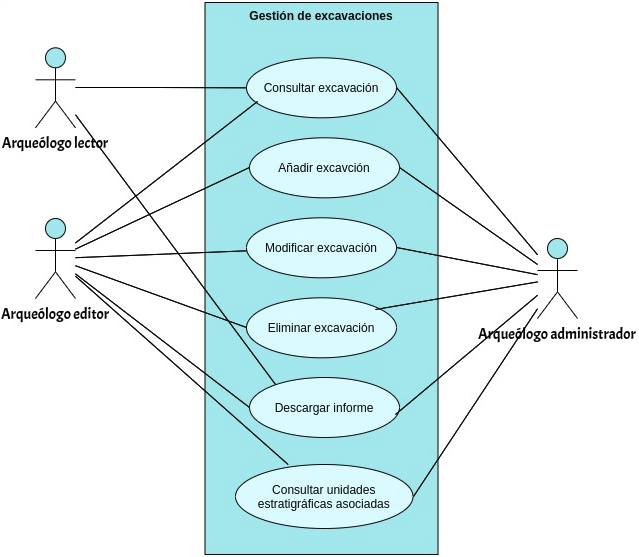
\includegraphics[scale=0.50]{imagenes/diagramas CU/excavation-UC.png}
        \caption{Gestión de excavaciones}
        \label{fig:excavation-management}
    \end{figure}

\subsubsection{Caso de uso 1.1: Consultar excavación}

    \begin{table}[H]
    \begin{center}
        \begin{adjustbox}{width=\textwidth}
        \begin{tabular}{ | l | l | l | l | c | c | } 
            \hline
            \textbf{Caso de uso} & \multicolumn{4}{l|}{Consultar excavación} & \cellcolor{gray!50} \textbf{CU-1.1}\\
            \hline
            \textbf{Actores} & \multicolumn{5}{p{0.5\linewidth}|}{Arqueólogo lector, arqueólogo editor, arqueólogo administrador} \\
            \hline
            \textbf{Tipo} & \multicolumn{5}{l|}{Primario y esencial} \\
            \hline
            \textbf{Referencias} & \multicolumn{3}{l|}{RF-1.1} & \multicolumn{2}{l|}{ }\\
            \hline
            \textbf{Precondición} & \multicolumn{5}{l|}{El usuario deberá estar registrado y activo en el sistema} \\
            \hline
            \textbf{Postcondición} & \multicolumn{5}{l|}{ } \\
            \hline
            \textbf{Autor} & \multicolumn{1}{p{0.25\linewidth}|}{Joaquín Alejandro España Sánchez} & \textbf{Fecha} & 
            17-02-2022     & \textbf{Versión}                                                      & 1.0\\
            \hline
        \end{tabular}
        \end{adjustbox}
        \caption{CU-1.1: Consultar excavación}
        \label{tab:consult-excavation}
    \end{center}
    \end{table}
    
    \begin{table}[H]
        \centering
        \begin{tabularx}{\textwidth}{@{} |L |@{}} \hline
            \rowcolor{gray!50} 
            \textbf{Propósito} \\
            \hline
            Permite al usuario visualizar el estado actual de una excavación. \\
            \hline
        \end{tabularx}
    \end{table}

    \begin{table}[H]
        \centering
        \begin{tabularx}{\textwidth}{@{} |L |@{}} \hline
            \rowcolor{gray!50} 
            \textbf{Resumen} \\
            \hline
            Permite a un determinado tipo de arqueólogo con permisos ver los datos asociados
            a una determinada excavación. \\
            \hline
        \end{tabularx}
    \end{table}

\subsubsection{Caso de uso 1.2: Añadir excavación}

\begin{table}[H]
    \begin{center}
        \begin{adjustbox}{width=\textwidth}
        \begin{tabular}{ | l | l | l | l | c | c | } 
            \hline
            \textbf{Caso de uso} & \multicolumn{4}{l|}{Añadir excavación} & \cellcolor{gray!50} \textbf{CU-1.2}\\
            \hline
            \textbf{Actores} & \multicolumn{5}{p{0.9\linewidth}|}{Arqueólogo editor, arqueólogo administrador } \\
            \hline
            \textbf{Tipo} & \multicolumn{5}{l|}{Primario y esencial} \\
            \hline
            \textbf{Referencias} & \multicolumn{3}{l|}{RF-1.2} & \multicolumn{2}{l|}{ }\\
            \hline
            \textbf{Precondición} & \multicolumn{5}{l|}{El usuario deberá estar registrado y activo en el sistema} \\
            \hline
            \textbf{Postcondición} & \multicolumn{5}{l|}{El usuario debe haber podido añadir una excavación nueva} \\
            \hline
            \textbf{Autor} & \multicolumn{1}{p{0.25\linewidth}|}{Joaquín Alejandro España Sánchez} & \textbf{Fecha} & 
            17-02-2022     & \textbf{Versión}                                                      & 1.0\\
            \hline
        \end{tabular}
        \end{adjustbox}
        \caption{CU-1.2: Añadir excavación}
        \label{tab:add-excavation}
    \end{center}
    \end{table}

    \begin{table}[H]
        \centering
        \begin{tabularx}{\textwidth}{@{} |L |@{}} \hline
            \rowcolor{gray!50} 
            \textbf{Propósito} \\
            \hline
            Permite al usuario añadir una nueva excavación en el sistema. \\
            \hline
        \end{tabularx}
    \end{table}

    \begin{table}[H]
        \centering
        \begin{tabularx}{\textwidth}{@{} |L |@{}} \hline
            \rowcolor{gray!50} 
            \textbf{Resumen} \\
            \hline
            Permite que un usuario pueda crear una nueva excavación en el sistema
            introduciendo los datos correspondientes en el formulario.\\
            \hline
        \end{tabularx}
    \end{table}

\subsubsection{Caso de uso 1.3: Modificar excavación}

    \begin{table}[H]
    \begin{center}
        \begin{adjustbox}{width=\textwidth}
        \begin{tabular}{ | l | l | l | l | c | c | } 
            \hline
            \textbf{Caso de uso} & \multicolumn{4}{l|}{Modificar excavación} & \cellcolor{gray!50} \textbf{CU-1.3}\\
            \hline
            \textbf{Actores} & \multicolumn{5}{p{0.9\linewidth}|}{Arqueólogo editor, arqueólogo administrador} \\
            \hline
            \textbf{Tipo} & \multicolumn{5}{l|}{Primario y esencial} \\
            \hline
            \textbf{Referencias} & \multicolumn{3}{l|}{RF-1.3} & \multicolumn{2}{l|}{ }\\
            \hline
            \textbf{Precondición} & \multicolumn{5}{l|}{El usuario deberá estar registrado y activo en el sistema} \\
            \hline
            \textbf{Postcondición} & \multicolumn{5}{l|}{El usuario debe haber podido modificar los datos relativos a la
            excavación} \\
            \hline
            \textbf{Autor} & \multicolumn{1}{p{0.25\linewidth}|}{Joaquín Alejandro España Sánchez} & \textbf{Fecha} & 
            17-02-2022     & \textbf{Versión}                                                      & 1.0\\
            \hline
        \end{tabular}
        \end{adjustbox}
        \caption{CU-1.3: Modificar excavación}
        \label{tab:modify-excavation}
    \end{center}
    \end{table}

    \begin{table}[H]
        \centering
        \begin{tabularx}{\textwidth}{@{} |L |@{}} \hline
            \rowcolor{gray!50} 
            \textbf{Propósito} \\
            \hline
            Sobreescribir la información de la excavación almacenada en el sistema. \\
            \hline
        \end{tabularx}
    \end{table}

    \begin{table}[H]
        \centering
        \begin{tabularx}{\textwidth}{@{} |L |@{}} \hline
            \rowcolor{gray!50} 
            \textbf{Resumen} \\
            \hline
            El arqueólogo editor o administrador modifica la información escrita
            anteriormente con respecto a una excavación.\\
            \hline
        \end{tabularx}
    \end{table}

\subsubsection{Caso de uso 1.4: Eliminar excavación}

    \begin{table}[H]
    \begin{center}
        \begin{adjustbox}{width=\textwidth}
        \begin{tabular}{ | l | l | l | l | c | c | } 
            \hline
            \textbf{Caso de uso} & \multicolumn{4}{l|}{Eliminar excavación} & \cellcolor{gray!50} \textbf{CU-1.4}\\
            \hline
            \textbf{Actores} & \multicolumn{5}{p{0.9\linewidth}|}{Arqueólogo editor, arqueólogo administrador} \\
            \hline
            \textbf{Tipo} & \multicolumn{5}{l|}{Primario y esencial} \\
            \hline
            \textbf{Referencias} & \multicolumn{3}{l|}{RF-1.4} & \multicolumn{2}{l|}{ }\\
            \hline
            \textbf{Precondición} & \multicolumn{5}{l|}{El usuario deberá estar registrado y activo en el sistema} \\
            \hline
            \textbf{Postcondición} & \multicolumn{5}{l|}{La excavación y toda la información asociada se eliminarán del
            sistema} \\
            \hline
            \textbf{Autor} & \multicolumn{1}{p{0.25\linewidth}|}{Joaquín Alejandro España Sánchez} & \textbf{Fecha} & 
            17-02-2022     & \textbf{Versión}                                                      & 1.0\\
            \hline
        \end{tabular}
        \end{adjustbox}
        \caption{CU-1.4: Eliminar excavación}
        \label{tab:delete-excavation}
    \end{center}
    \end{table}

    \begin{table}[H]
        \centering
        \begin{tabularx}{\textwidth}{@{} |L |@{}} \hline
            \rowcolor{gray!50} 
            \textbf{Propósito} \\
            \hline
            Permite a un usuario eliminar cualquier información asociada a una excavación. \\
            \hline
        \end{tabularx}
    \end{table}

    \begin{table}[H]
        \centering
        \begin{tabularx}{\textwidth}{@{} |L |@{}} \hline
            \rowcolor{gray!50} 
            \textbf{Resumen} \\
            \hline
            El arqueólogo editor o administrador con permisos podrá eliminar una determinada
            excavación previamente almacenada en el sistema. \\
            \hline
        \end{tabularx}
    \end{table}

\subsubsection{Caso de uso 1.5: Descargar informe}

    \begin{table}[H]
    \begin{center}
        \begin{adjustbox}{width=\textwidth}
        \begin{tabular}{ | l | l | l | l | c | c | } 
            \hline
            \textbf{Caso de uso} & \multicolumn{4}{l|}{Descargar informe} & \cellcolor{gray!50} \textbf{CU-1.5}\\
            \hline
            \textbf{Actores} & \multicolumn{5}{p{0.9\linewidth}|}{Arqueólogo editor, arqueólogo administrador} \\
            \hline
            \textbf{Tipo} & \multicolumn{5}{l|}{Primario y esencial} \\
            \hline
            \textbf{Referencias} & \multicolumn{3}{l|}{RF-1.5} & \multicolumn{2}{l|}{ }\\
            \hline
            \textbf{Precondición} & \multicolumn{5}{l|}{El usuario deberá estar registrado y activo en el sistema} \\
            \hline
            \textbf{Postcondición} & \multicolumn{5}{p{1.0\linewidth}|}{El usuario habrá podido descargar un documento editable con toda
            la información asociada a una excavación concreta} \\
            \hline
            \textbf{Autor} & \multicolumn{1}{p{0.25\linewidth}|}{Joaquín Alejandro España Sánchez} & \textbf{Fecha} & 
            17-02-2022     & \textbf{Versión}                                                      & 1.0\\
            \hline
        \end{tabular}
        \end{adjustbox}
        \caption{CU-1.5: Descargar informe}
        \label{tab:download-report}
    \end{center}
    \end{table}

    \begin{table}[H]
        \centering
        \begin{tabularx}{\textwidth}{@{} |L |@{}} \hline
            \rowcolor{gray!50} 
            \textbf{Propósito} \\
            \hline
            Permite generar y descargar un informe asociado a una excavación. \\
            \hline
        \end{tabularx}
    \end{table}

    \begin{table}[H]
        \centering
        \begin{tabularx}{\textwidth}{@{} |L |@{}} \hline
            \rowcolor{gray!50} 
            \textbf{Resumen} \\
            \hline
            El usuario podrá descargar toda la información asociada a una excavación
            concreta seleccionando la opción de \textit{descargar informe} de las
            opciones disponibles. \\
            \hline
        \end{tabularx}
    \end{table}

\subsubsection{Caso de uso 1.6: Consultar unidades estratigráficas asociadas}

    \begin{table}[H]
    \begin{center}
        \begin{adjustbox}{width=\textwidth}
        \begin{tabular}{ | l | l | l | l | c | c | } 
            \hline
            \textbf{Caso de uso} & \multicolumn{4}{l|}{Consultar unidades estratigráficas asociadas} & \cellcolor{gray!50} \textbf{CU-1.6}\\
            \hline
            \textbf{Actores} & \multicolumn{5}{p{0.9\linewidth}|}{Arqueólogo lector, arqueólogo editor, arqueólogo administrador} \\
            \hline
            \textbf{Tipo} & \multicolumn{5}{l|}{Primario y esencial} \\
            \hline
            \textbf{Referencias} & \multicolumn{3}{l|}{RF-1.6} & \multicolumn{2}{l|}{CU-4.1}\\
            \hline
            \textbf{Precondición} & \multicolumn{5}{l|}{El usuario deberá estar registrado y activo en el sistema} \\
            \hline
            \textbf{Postcondición} & \multicolumn{5}{l|}{ } \\
            \hline
            \textbf{Autor} & \multicolumn{1}{p{0.25\linewidth}|}{Joaquín Alejandro España Sánchez} & \textbf{Fecha} & 
            17-02-2022     & \textbf{Versión}                                                      & 1.0\\
            \hline
        \end{tabular}
        \end{adjustbox}
        \caption{CU-1.6: Consultar unidades estratigráficas asociadas}
        \label{tab:consult-ues-excavation}
    \end{center}
    \end{table}

    \begin{table}[H]
        \centering
        \begin{tabularx}{\textwidth}{@{} |L |@{}} \hline
            \rowcolor{gray!50} 
            \textbf{Propósito} \\
            \hline
            Consultar las unidades estratigráficas que pertenecen a una excavación. \\
            \hline
        \end{tabularx}
    \end{table}

    \begin{table}[H]
        \centering
        \begin{tabularx}{\textwidth}{@{} |L |@{}} \hline
            \rowcolor{gray!50} 
            \textbf{Resumen} \\
            \hline
            El usuario podrá visualizar las unidades estratigráficas que están asociadas
            a una determinada excavación, que podrán ser tanto sedimentarias como
            construidas. \\
            \hline
        \end{tabularx}
    \end{table}

% ESTANCIA
\subsection{Gestión de estancias}
    \begin{figure}[H]
        \centering
        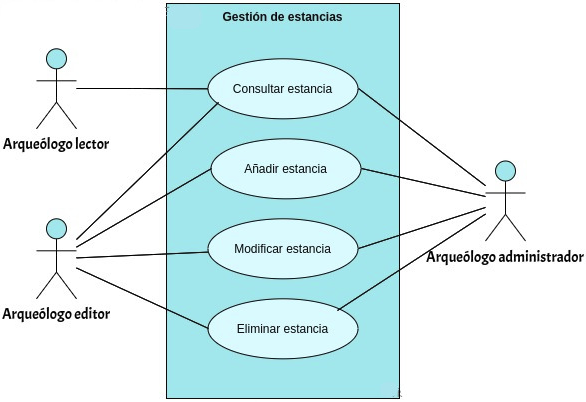
\includegraphics[scale=0.40]{imagenes/diagramas CU/room-UC.png}
        \caption{Gestión de estancias}
        \label{fig:room-management}
    \end{figure}

\subsubsection{Caso de uso 2.1: Consultar estancia}

    \begin{table}[H]
    \begin{center}
        \begin{adjustbox}{width=\textwidth}
        \begin{tabular}{ | l | l | l | l | c | c | } 
            \hline
            \textbf{Caso de uso} & \multicolumn{4}{l|}{Consultar estancia} & \cellcolor{gray!50} \textbf{CU-2.1}\\
            \hline
            \textbf{Actores} & \multicolumn{5}{p{0.9\linewidth}|}{Arqueólogo lector, arqueólogo editor, arqueólogo administrador} \\
            \hline
            \textbf{Tipo} & \multicolumn{5}{l|}{Primario y esencial} \\
            \hline
            \textbf{Referencias} & \multicolumn{3}{l|}{RF-2.1} & \multicolumn{2}{l|}{ }\\
            \hline
            \textbf{Precondición} & \multicolumn{5}{l|}{El usuario deberá estar registrado y activo en el sistema} \\
            \hline
            \textbf{Postcondición} & \multicolumn{5}{l|}{ } \\
            \hline
            \textbf{Autor} & \multicolumn{1}{p{0.25\linewidth}|}{Joaquín Alejandro España Sánchez} & \textbf{Fecha} & 
            17-02-2022     & \textbf{Versión}                                                      & 1.0\\
            \hline
        \end{tabular}
        \end{adjustbox}
        \caption{CU-2.1: Consultar estancia}
        \label{tab:consult-room}
    \end{center}
    \end{table}

    \begin{table}[H]
        \centering
        \begin{tabularx}{\textwidth}{@{} |L |@{}} \hline
            \rowcolor{gray!50} 
            \textbf{Propósito} \\
            \hline
            Permite al usuario visualizar el estado actual de una estancia. \\
            \hline
        \end{tabularx}
    \end{table}

    \begin{table}[H]
        \centering
        \begin{tabularx}{\textwidth}{@{} |L |@{}} \hline
            \rowcolor{gray!50} 
            \textbf{Resumen} \\
            \hline
            Permite a un determinado tipo de arqueólogo con permisos ver los datos asociados
            a una determinada estancia. \\
            \hline
        \end{tabularx}
    \end{table}

\subsubsection{Caso de uso 2.2: Añadir estancia}

    \begin{table}[H]
    \begin{center}
        \begin{adjustbox}{width=\textwidth}
        \begin{tabular}{ | l | l | l | l | c | c | } 
            \hline
            \textbf{Caso de uso} & \multicolumn{4}{l|}{Añadir estancia} & \cellcolor{gray!50} \textbf{CU-2.2}\\
            \hline
            \textbf{Actores} & \multicolumn{5}{p{0.9\linewidth}|}{Arqueólogo editor, arqueólogo administrador} \\
            \hline
            \textbf{Tipo} & \multicolumn{5}{l|}{Primario y esencial} \\
            \hline
            \textbf{Referencias} & \multicolumn{3}{l|}{RF-2.2} & \multicolumn{2}{l|}{ }\\
            \hline
            \textbf{Precondición} & \multicolumn{5}{l|}{El usuario deberá estar registrado y activo en el sistema} \\
            \hline
            \textbf{Postcondición} & \multicolumn{5}{l|}{El usuario debe haber podido añadir una estancia nueva} \\
            \hline
            \textbf{Autor} & \multicolumn{1}{p{0.25\linewidth}|}{Joaquín Alejandro España Sánchez} & \textbf{Fecha} & 
            17-02-2022     & \textbf{Versión}                                                      & 1.0\\
            \hline
        \end{tabular}
        \end{adjustbox}
        \caption{CU-2.2: Añadir estancia}
        \label{tab:add-room}
    \end{center}
    \end{table}

    \begin{table}[H]
        \centering
        \begin{tabularx}{\textwidth}{@{} |L |@{}} \hline
            \rowcolor{gray!50} 
            \textbf{Propósito} \\
            \hline
            Permite a un usuario añadir una nueva estancia al sistema. \\
            \hline
        \end{tabularx}
    \end{table}

    \begin{table}[H]
        \centering
        \begin{tabularx}{\textwidth}{@{} |L |@{}} \hline
            \rowcolor{gray!50} 
            \textbf{Resumen} \\
            \hline
            Permite almacenar una nueva estancia en el sistema tras introducir los datos
            necesarios de la estancia en el formulario correspondiente.\\
            \hline
        \end{tabularx}
    \end{table}

\subsubsection{Caso de uso 2.3: Modificar estancia}

    \begin{table}[H]
    \begin{center}
        \begin{adjustbox}{width=\textwidth}
        \begin{tabular}{ | l | l | l | l | c | c | } 
            \hline
            \textbf{Caso de uso} & \multicolumn{4}{l|}{Modificar estancia} & \cellcolor{gray!50} \textbf{CU-2.3}\\
            \hline
            \textbf{Actores} & \multicolumn{5}{p{0.9\linewidth}|}{Arqueólogo editor, arqueólogo administrador} \\
            \hline
            \textbf{Tipo} & \multicolumn{5}{l|}{Primario y esencial} \\
            \hline
            \textbf{Referencias} & \multicolumn{3}{l|}{RF-1.1} & \multicolumn{2}{l|}{ }\\
            \hline
            \textbf{Precondición} & \multicolumn{5}{l|}{El usuario deberá estar registrado y activo en el sistema} \\
            \hline
            \textbf{Postcondición} & \multicolumn{5}{l|}{El usuario debe haber podido modificar los datos relativos a la
            estancia} \\
            \hline
            \textbf{Autor} & \multicolumn{1}{p{0.25\linewidth}|}{Joaquín Alejandro España Sánchez} & \textbf{Fecha} & 
            17-02-2022     & \textbf{Versión}                                                      & 1.0\\
            \hline
        \end{tabular}
        \end{adjustbox}
        \caption{CU-2.3: Modificar estancia}
        \label{tab:modify-room}
    \end{center}
    \end{table}

    \begin{table}[H]
        \centering
        \begin{tabularx}{\textwidth}{@{} |L |@{}} \hline
            \rowcolor{gray!50} 
            \textbf{Propósito} \\
            \hline
            Sobreescribir la información de una estancia almacenada en el sistema. \\
            \hline
        \end{tabularx}
    \end{table}

    \begin{table}[H]
        \centering
        \begin{tabularx}{\textwidth}{@{} |L |@{}} \hline
            \rowcolor{gray!50} 
            \textbf{Resumen} \\
            \hline
            El arqueólogo editor o administrador modifica la información almacenada
            anteriormente de una estancia.\\
            \hline
        \end{tabularx}
    \end{table}

\subsubsection{Caso de uso 2.4: Eliminar estancia}

    \begin{table}[H]
    \begin{center}
        \begin{adjustbox}{width=\textwidth}
        \begin{tabular}{ | l | l | l | l | c | c | } 
            \hline
            \textbf{Caso de uso} & \multicolumn{4}{l|}{Consultar excavación} & \cellcolor{gray!50} \textbf{CU-2.4}\\
            \hline
            \textbf{Actores} & \multicolumn{5}{p{0.9\linewidth}|}{Arqueólogo editor, arqueólogo administrador} \\
            \hline
            \textbf{Tipo} & \multicolumn{5}{l|}{Primario y esencial} \\
            \hline
            \textbf{Referencias} & \multicolumn{3}{l|}{RF-2.4} & \multicolumn{2}{l|}{ }\\
            \hline
            \textbf{Precondición} & \multicolumn{5}{l|}{El usuario deberá estar registrado y activo en el sistema} \\
            \hline
            \textbf{Postcondición} & \multicolumn{5}{l|}{La estancia y toda la información asociada se eliminarán del sistema} \\
            \hline
            \textbf{Autor} & \multicolumn{1}{p{0.25\linewidth}|}{Joaquín Alejandro España Sánchez} & \textbf{Fecha} & 
            17-02-2022     & \textbf{Versión}                                                      & 1.0\\
            \hline
        \end{tabular}
        \end{adjustbox}
        \caption{CU-2.4: Eliminar estancia}
        \label{tab:delete-room}
    \end{center}
    \end{table}


    \begin{table}[H]
        \centering
        \begin{tabularx}{\textwidth}{@{} |L |@{}} \hline
            \rowcolor{gray!50} 
            \textbf{Propósito} \\
            \hline
            Permite a un usuario eliminar cualquier información asociada a una estancia. \\
            \hline
        \end{tabularx}
    \end{table}

    \begin{table}[H]
        \centering
        \begin{tabularx}{\textwidth}{@{} |L |@{}} \hline
            \rowcolor{gray!50} 
            \textbf{Resumen} \\
            \hline
            El arqueólogo editor o administrador con permisos podrá eliminar una determinada
            estancia previamente almacenada en el sistema. \\
            \hline
        \end{tabularx}
    \end{table}

% HECHOS
\subsection{Gestión de hechos}
    \begin{figure}[H]
        \centering
        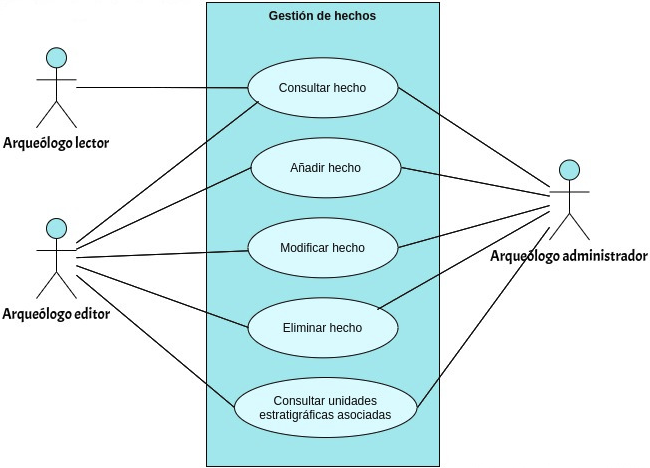
\includegraphics[scale=0.50]{imagenes/diagramas CU/fact-UC.png}
        \caption{Gestión de hechos}
        \label{fig:fact-management}
    \end{figure}

\subsubsection{Caso de uso 3.1: Consultar hecho}

    \begin{table}[H]
    \begin{center}
        \begin{adjustbox}{width=\textwidth}
        \begin{tabular}{ | l | l | l | l | c | c | } 
            \hline
            \textbf{Caso de uso} & \multicolumn{4}{l|}{Consultar hecho} & \cellcolor{gray!50} \textbf{CU-3.1}\\
            \hline
            \textbf{Actores} & \multicolumn{5}{p{0.9\linewidth}|}{Arqueólogo lector, arqueólogo editor, arqueólogo administrador} \\
            \hline
            \textbf{Tipo} & \multicolumn{5}{l|}{Primario y esencial} \\
            \hline
            \textbf{Referencias} & \multicolumn{3}{l|}{RF-3.1} & \multicolumn{2}{l|}{ }\\
            \hline
            \textbf{Precondición} & \multicolumn{5}{l|}{El usuario deberá estar registrado y activo en el sistema} \\
            \hline
            \textbf{Postcondición} & \multicolumn{5}{l|}{ } \\
            \hline
            \textbf{Autor} & \multicolumn{1}{p{0.25\linewidth}|}{Joaquín Alejandro España Sánchez} & \textbf{Fecha} & 
            17-02-2022     & \textbf{Versión}                                                      & 1.0\\
            \hline
        \end{tabular}
        \end{adjustbox}
        \caption{CU-3.1: Consultar hecho}
        \label{tab:consult-fact}
    \end{center}
    \end{table}

    \begin{table}[H]
        \centering
        \begin{tabularx}{\textwidth}{@{} |L |@{}} \hline
            \rowcolor{gray!50} 
            \textbf{Propósito} \\
            \hline
            Permite al usuario visualizar el estado actual de un hecho. \\
            \hline
        \end{tabularx}
    \end{table}

    \begin{table}[H]
        \centering
        \begin{tabularx}{\textwidth}{@{} |L |@{}} \hline
            \rowcolor{gray!50} 
            \textbf{Resumen} \\
            \hline
            Permite a un determinado tipo de arqueólogo con permisos ver los datos asociados
            a un determinado hecho. \\
            \hline
        \end{tabularx}
    \end{table}

\subsubsection{Caso de uso 3.2: Añadir hecho}

    \begin{table}[H]
    \begin{center}
        \begin{adjustbox}{width=\textwidth}
        \begin{tabular}{ | l | l | l | l | c | c | } 
            \hline
            \textbf{Caso de uso} & \multicolumn{4}{l|}{Añadir hecho} & \cellcolor{gray!50} \textbf{CU-3.2}\\
            \hline
            \textbf{Actores} & \multicolumn{5}{p{0.9\linewidth}|}{Arqueólogo editor, arqueólogo administrador} \\
            \hline
            \textbf{Tipo} & \multicolumn{5}{l|}{Primario y esencial} \\
            \hline
            \textbf{Referencias} & \multicolumn{3}{l|}{RF-3.2} & \multicolumn{2}{l|}{ }\\
            \hline
            \textbf{Precondición} & \multicolumn{5}{l|}{El usuario deberá estar registrado y activo en el sistema} \\
            \hline
            \textbf{Postcondición} & \multicolumn{5}{l|}{El usuario debe haber podido añadir un hecho nuevo} \\
            \hline
            \textbf{Autor} & \multicolumn{1}{p{0.25\linewidth}|}{Joaquín Alejandro España Sánchez} & \textbf{Fecha} & 
            17-02-2022     & \textbf{Versión}                                                      & 1.0\\
            \hline
        \end{tabular}
        \end{adjustbox}
        \caption{CU-3.2: Añadir hecho}
        \label{tab:add-fact}
    \end{center}
    \end{table}

    \begin{table}[H]
        \centering
        \begin{tabularx}{\textwidth}{@{} |L |@{}} \hline
            \rowcolor{gray!50} 
            \textbf{Propósito} \\
            \hline
            Permite a un usuario añadir un nuevo hecho al sistema. \\
            \hline
        \end{tabularx}
    \end{table}

    \begin{table}[H]
        \centering
        \begin{tabularx}{\textwidth}{@{} |L |@{}} \hline
            \rowcolor{gray!50} 
            \textbf{Resumen} \\
            \hline
            Permite almacenar un nuevo hecho en el sistema tras introducir los datos
            necesarios del hecho en el formulario correspondiente.\\
            \hline
        \end{tabularx}
    \end{table}

\subsubsection{Caso de uso 3.3: Modificar hecho}

    \begin{table}[H]
    \begin{center}
        \begin{adjustbox}{width=\textwidth}
        \begin{tabular}{ | l | l | l | l | c | c | } 
            \hline
            \textbf{Caso de uso} & \multicolumn{4}{l|}{Modificar hecho} & \cellcolor{gray!50} \textbf{CU-3.3}\\
            \hline
            \textbf{Actores} & \multicolumn{5}{p{0.9\linewidth}|}{Arqueólogo editor, arqueólogo administrador} \\
            \hline
            \textbf{Tipo} & \multicolumn{5}{l|}{Primario y esencial} \\
            \hline
            \textbf{Referencias} & \multicolumn{3}{l|}{RF-1.1} & \multicolumn{2}{l|}{ }\\
            \hline
            \textbf{Precondición} & \multicolumn{5}{l|}{El usuario deberá estar registrado y activo en el sistema} \\
            \hline
            \textbf{Postcondición} & \multicolumn{5}{l|}{El usuario debe haber podido modificar los datos relativos al hecho} \\
            \hline
            \textbf{Autor} & \multicolumn{1}{p{0.25\linewidth}|}{Joaquín Alejandro España Sánchez} & \textbf{Fecha} & 
            17-02-2022     & \textbf{Versión}                                                      & 1.0\\
            \hline
        \end{tabular}
        \end{adjustbox}
        \caption{CU-3.3: Modificar hecho}
        \label{tab:modify-fact}
    \end{center}
    \end{table}

    \begin{table}[H]
        \centering
        \begin{tabularx}{\textwidth}{@{} |L |@{}} \hline
            \rowcolor{gray!50} 
            \textbf{Propósito} \\
            \hline
            Sobreescribir la información de un hecho almacenado en el sistema. \\
            \hline
        \end{tabularx}
    \end{table}

    \begin{table}[H]
        \centering
        \begin{tabularx}{\textwidth}{@{} |L |@{}} \hline
            \rowcolor{gray!50} 
            \textbf{Resumen} \\
            \hline
            El arqueólogo editor o administrador modifica la información almacenada
            anteriormente de un hecho.\\
            \hline
        \end{tabularx}
    \end{table}

\subsubsection{Caso de uso 3.4: Eliminar hecho}

    \begin{table}[H]
    \begin{center}
        \begin{adjustbox}{width=\textwidth}
        \begin{tabular}{ | l | l | l | l | c | c | } 
            \hline
            \textbf{Caso de uso} & \multicolumn{4}{l|}{Eliminar hecho} & \cellcolor{gray!50} \textbf{CU-3.4}\\
            \hline
            \textbf{Actores} & \multicolumn{5}{p{0.9\linewidth}|}{Arqueólogo editor, arqueólogo administrador} \\
            \hline
            \textbf{Tipo} & \multicolumn{5}{l|}{Primario y esencial} \\
            \hline
            \textbf{Referencias} & \multicolumn{3}{l|}{RF-3.4} & \multicolumn{2}{l|}{ }\\
            \hline
            \textbf{Precondición} & \multicolumn{5}{l|}{El usuario deberá estar registrado y activo en el sistema} \\
            \hline
            \textbf{Postcondición} & \multicolumn{5}{l|}{El hecho y toda la información asociada se eliminarán del sistema} \\
            \hline
            \textbf{Autor} & \multicolumn{1}{p{0.25\linewidth}|}{Joaquín Alejandro España Sánchez} & \textbf{Fecha} & 
            17-02-2022     & \textbf{Versión}                                                      & 1.0\\
            \hline
        \end{tabular}
        \end{adjustbox}
        \caption{CU-3.4: Eliminar hecho}
        \label{tab:delete-fact}
    \end{center}
    \end{table}

    \begin{table}[H]
        \centering
        \begin{tabularx}{\textwidth}{@{} |L |@{}} \hline
            \rowcolor{gray!50} 
            \textbf{Propósito} \\
            \hline
            Permite a un usuario eliminar cualquier información asociada a un hecho. \\
            \hline
        \end{tabularx}
    \end{table}

    \begin{table}[H]
        \centering
        \begin{tabularx}{\textwidth}{@{} |L |@{}} \hline
            \rowcolor{gray!50} 
            \textbf{Resumen} \\
            \hline
            El arqueólogo editor o administrador con permisos podrá eliminar un determinado
            hecho previamente almacenado en el sistema. \\
            \hline
        \end{tabularx}
    \end{table}

\subsubsection{Caso de uso 3.5: Consultar unidades estratigráficas asociadas}

    \begin{table}[H]
    \begin{center}
        \begin{adjustbox}{width=\textwidth}
        \begin{tabular}{ | l | l | l | l | c | c | } 
            \hline
            \textbf{Caso de uso} & \multicolumn{4}{l|}{Consultar unidades estratigráficas asociadas} & \cellcolor{gray!50} \textbf{CU-3.5}\\
            \hline
            \textbf{Actores} & \multicolumn{5}{p{0.9\linewidth}|}{Arqueólogo lector, arqueólogo editor, arqueólogo administrador} \\
            \hline
            \textbf{Tipo} & \multicolumn{5}{l|}{Primario y esencial} \\
            \hline
            \textbf{Referencias} & \multicolumn{3}{l|}{RF-3.5} & \multicolumn{2}{l|}{CU-4.1}\\
            \hline
            \textbf{Precondición} & \multicolumn{5}{l|}{El usuario deberá estar registrado y activo en el sistema} \\
            \hline
            \textbf{Postcondición} & \multicolumn{5}{l|}{} \\
            \hline
            \textbf{Autor} & \multicolumn{1}{p{0.25\linewidth}|}{Joaquín Alejandro España Sánchez} & \textbf{Fecha} & 
            17-02-2022     & \textbf{Versión}                                                      & 1.0\\
            \hline
        \end{tabular}
        \end{adjustbox}
        \caption{CU-3.5: Consultar unidades estratigráficas asociadas}
        \label{tab:consult-ue-fact}
    \end{center}
    \end{table}

    \begin{table}[H]
        \centering
        \begin{tabularx}{\textwidth}{@{} |L |@{}} \hline
            \rowcolor{gray!50} 
            \textbf{Propósito} \\
            \hline
            Consultar las unidades estratigráficas que pertenecen a un hecho. \\
            \hline
        \end{tabularx}
    \end{table}

    \begin{table}[H]
        \centering
        \begin{tabularx}{\textwidth}{@{} |L |@{}} \hline
            \rowcolor{gray!50} 
            \textbf{Resumen} \\
            \hline
            El usuario podrá visualizar las unidades estratigráficas que están asociadas
            a un determinado hecho, que podrán ser tanto sedimentarias como construidas. \\
            \hline
        \end{tabularx}
    \end{table}


% UNIDADES ESTRATIGRÁFICAS
\subsection{Gestión de unidades estratigráficas}
    \begin{figure}[H]
        \centering
        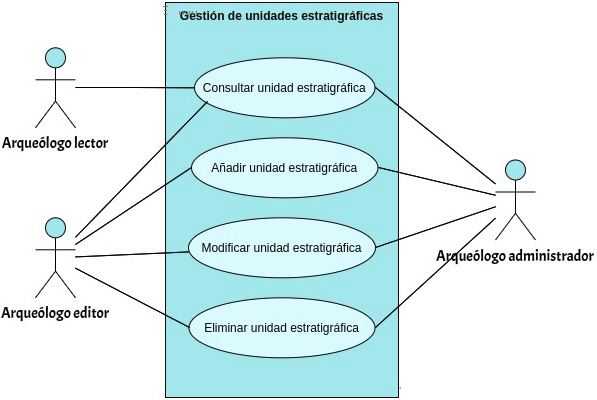
\includegraphics[scale=0.50]{imagenes/diagramas CU/UE-UC.png}
        \caption{Gestión de unidades estratigráficas}
        \label{fig:ue-management}
    \end{figure}

\subsubsection{Caso de uso 4.1: Consultar unidad estratigráfica}

    \begin{table}[H]
    \begin{center}
        \begin{adjustbox}{width=\textwidth}
        \begin{tabular}{ | l | l | l | l | c | c | } 
            \hline
            \textbf{Caso de uso} & \multicolumn{4}{l|}{Consultar unidad estratigráfica} & \cellcolor{gray!50} \textbf{CU-4.1}\\
            \hline
            \textbf{Actores} & \multicolumn{5}{p{0.9\linewidth}|}{Arqueólogo lector, arqueólogo editor, arqueólogo administrador} \\
            \hline
            \textbf{Tipo} & \multicolumn{5}{l|}{Primario y esencial} \\
            \hline
            \textbf{Referencias} & \multicolumn{3}{l|}{RF-4.1} & \multicolumn{2}{l|}{ }\\
            \hline
            \textbf{Precondición} & \multicolumn{5}{l|}{El usuario deberá estar registrado y activo en el sistema} \\
            \hline
            \textbf{Postcondición} & \multicolumn{5}{l|}{ } \\
            \hline
            \textbf{Autor} & \multicolumn{1}{p{0.25\linewidth}|}{Joaquín Alejandro España Sánchez} & \textbf{Fecha} & 
            17-02-2022     & \textbf{Versión}                                                      & 1.0\\
            \hline
        \end{tabular}
        \end{adjustbox}
        \caption{CU-4.1: Consultar unidad estratigráfica}
        \label{tab:consult-ue}
    \end{center}
    \end{table}


    \begin{table}[H]
        \centering
        \begin{tabularx}{\textwidth}{@{} |L |@{}} \hline
            \rowcolor{gray!50} 
            \textbf{Propósito} \\
            \hline
            Permite al usuario visualizar el estado actual de una unidad estratigráfica
            (sedimentaria o costruida). \\
            \hline
        \end{tabularx}
    \end{table}

    \begin{table}[H]
        \centering
        \begin{tabularx}{\textwidth}{@{} |L |@{}} \hline
            \rowcolor{gray!50} 
            \textbf{Resumen} \\
            \hline
            Permite a un determinado tipo de arqueólogo con permisos ver los datos asociados
            a una determinada unidad estratigráfica (sedimentaria o construida). \\
            \hline
        \end{tabularx}
    \end{table}

\subsubsection{Caso de uso 4.2: Añadir unidad estratigráfica}

    \begin{table}[H]
    \begin{center}
        \begin{adjustbox}{width=\textwidth}
        \begin{tabular}{ | l | l | l | l | c | c | } 
            \hline
            \textbf{Caso de uso} & \multicolumn{4}{l|}{Añadir unidad estratigráfica} & \cellcolor{gray!50} \textbf{CU-4.2}\\
            \hline
            \textbf{Actores} & \multicolumn{5}{p{0.9\linewidth}|}{Arqueólogo editor, arqueólogo administrador} \\
            \hline
            \textbf{Tipo} & \multicolumn{5}{l|}{Primario y esencial} \\
            \hline
            \textbf{Referencias} & \multicolumn{3}{l|}{RF-4.2} & \multicolumn{2}{l|}{ }\\
            \hline
            \textbf{Precondición} & \multicolumn{5}{l|}{El usuario deberá estar registrado y activo en el sistema} \\
            \hline
            \textbf{Postcondición} & \multicolumn{5}{l|}{El usuario debe haber podido añadir una unidad estratigráfica nueva} \\
            \hline
            \textbf{Autor} & \multicolumn{1}{p{0.25\linewidth}|}{Joaquín Alejandro España Sánchez} & \textbf{Fecha} & 
            17-02-2022     & \textbf{Versión}                                                      & 1.0\\
            \hline
        \end{tabular}
        \end{adjustbox}
        \caption{CU-4.2: Añadir unidad estratigráfica}
        \label{tab:add-ue}
    \end{center}
    \end{table}

    \begin{table}[H]
        \centering
        \begin{tabularx}{\textwidth}{@{} |L |@{}} \hline
            \rowcolor{gray!50} 
            \textbf{Propósito} \\
            \hline
            Permite a un usuario añadir una nueva unidad estratigráfica al sistema. \\
            \hline
        \end{tabularx}
    \end{table}

    \begin{table}[H]
        \centering
        \begin{tabularx}{\textwidth}{@{} |L |@{}} \hline
            \rowcolor{gray!50} 
            \textbf{Resumen} \\
            \hline
            Permite almacenar una nueva unidad estratigráfica en el sistema tras introducir
            los datos necesarios de la estancia en el formulario correspondiente.\\
            \hline
        \end{tabularx}
    \end{table}

\subsubsection{Caso de uso 4.3: Modificar unidad estratigráfica}

    \begin{table}[H]
    \begin{center}
        \begin{adjustbox}{width=\textwidth}
        \begin{tabular}{ | l | l | l | l | c | c | } 
            \hline
            \textbf{Caso de uso} & \multicolumn{4}{l|}{Modificar unidad estratigráfica} & \cellcolor{gray!50} \textbf{CU-4.3}\\
            \hline
            \textbf{Actores} & \multicolumn{5}{p{0.9\linewidth}|}{Arqueólogo editor, arqueólogo administrador} \\
            \hline
            \textbf{Tipo} & \multicolumn{5}{l|}{Primario y esencial} \\
            \hline
            \textbf{Referencias} & \multicolumn{3}{l|}{RF-4.3} & \multicolumn{2}{l|}{ }\\
            \hline
            \textbf{Precondición} & \multicolumn{5}{l|}{El usuario deberá estar registrado y activo en el sistema} \\
            \hline
            \textbf{Postcondición} & \multicolumn{5}{l|}{El usuario debe haber podido modificar los datos relativos a la
            unidad estratigráfica} \\
            \hline
            \textbf{Autor} & \multicolumn{1}{p{0.25\linewidth}|}{Joaquín Alejandro España Sánchez} & \textbf{Fecha} & 
            17-02-2022     & \textbf{Versión}                                                      & 1.0\\
            \hline
        \end{tabular}
        \end{adjustbox}
        \caption{CU-4.3: Modificar unidad estratigráfica}
        \label{tab:modify-ue}
    \end{center}
    \end{table}

    \begin{table}[H]
        \centering
        \begin{tabularx}{\textwidth}{@{} |L |@{}} \hline
            \rowcolor{gray!50} 
            \textbf{Propósito} \\
            \hline
            Sobreescribir la información de una unidad estratigráfica almacenada en el sistema. \\
            \hline
        \end{tabularx}
    \end{table}

    \begin{table}[H]
        \centering
        \begin{tabularx}{\textwidth}{@{} |L |@{}} \hline
            \rowcolor{gray!50} 
            \textbf{Resumen} \\
            \hline
            El arqueólogo editor o administrador modifica la información almacenada
            anteriormente de una unidad estratigráfica.\\
            \hline
        \end{tabularx}
    \end{table}

\subsubsection{Caso de uso 4.4: Eliminar unidad estratigráfica}

    \begin{table}[H]
    \begin{center}
        \begin{adjustbox}{width=\textwidth}
        \begin{tabular}{ | l | l | l | l | c | c | } 
            \hline
            \textbf{Caso de uso} & \multicolumn{4}{l|}{Eliminar unidad estratigráfica} & \cellcolor{gray!50} \textbf{CU-4.4}\\
            \hline
            \textbf{Actores} & \multicolumn{5}{p{0.9\linewidth}|}{Arqueólogo editor, arqueólogo administrador} \\
            \hline
            \textbf{Tipo} & \multicolumn{5}{l|}{Primario y esencial} \\
            \hline
            \textbf{Referencias} & \multicolumn{3}{l|}{RF-4.4} & \multicolumn{2}{l|}{ }\\
            \hline
            \textbf{Precondición} & \multicolumn{5}{l|}{El usuario deberá estar registrado y activo en el sistema} \\
            \hline
            \textbf{Postcondición} & \multicolumn{5}{l|}{La unidad estratigráfica y toda la información asociada se
            eliminarán del sistema} \\
            \hline
            \textbf{Autor} & \multicolumn{1}{p{0.25\linewidth}|}{Joaquín Alejandro España Sánchez} & \textbf{Fecha} & 
            17-02-2022     & \textbf{Versión}                                                      & 1.0\\
            \hline
        \end{tabular}
        \end{adjustbox}
        \caption{CU-4.4: Eliminar unidad estratigráfica}
        \label{tab:delete-ue}
    \end{center}
    \end{table}

    \begin{table}[H]
        \centering
        \begin{tabularx}{\textwidth}{@{} |L |@{}} \hline
            \rowcolor{gray!50} 
            \textbf{Propósito} \\
            \hline
            Permite a un usuario eliminar cualquier información asociada a una unidad
            estratigráfica. \\
            \hline
        \end{tabularx}
    \end{table}

    \begin{table}[H]
        \centering
        \begin{tabularx}{\textwidth}{@{} |L |@{}} \hline
            \rowcolor{gray!50} 
            \textbf{Resumen} \\
            \hline
            El arqueólogo editor o administrador con permisos podrá eliminar una determinada
            unidad estratigráfica previamente almacenada en el sistema. \\
            \hline
        \end{tabularx}
    \end{table}

% FOTOGRAFIA
\subsection{Gestión de inventario fotográfico}
    \begin{figure}[H]
        \centering
        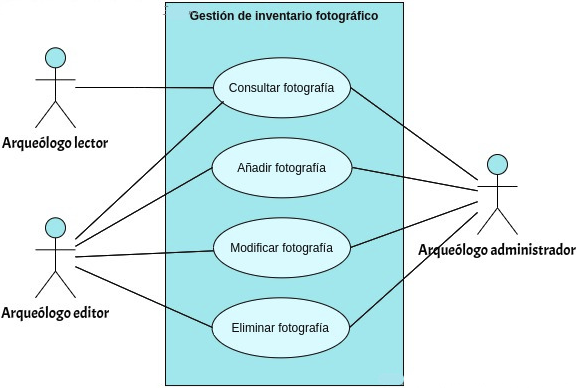
\includegraphics[scale=0.60]{imagenes/diagramas CU/photo-UC.png}
        \caption{Gestión de fotografías}
        \label{fig:photo-management}
    \end{figure}

\subsubsection{Caso de uso 5.1: Consultar fotografía}

    \begin{table}[H]
    \begin{center}
        \begin{adjustbox}{width=\textwidth}
        \begin{tabular}{ | l | l | l | l | c | c | } 
            \hline
            \textbf{Caso de uso} & \multicolumn{4}{l|}{Consultar fotografía} & \cellcolor{gray!50} \textbf{CU-5.1}\\
            \hline
            \textbf{Actores} & \multicolumn{5}{p{0.9\linewidth}|}{Arqueólogo lector, arqueólogo editor, arqueólogo administrador} \\
            \hline
            \textbf{Tipo} & \multicolumn{5}{l|}{Primario y esencial} \\
            \hline
            \textbf{Referencias} & \multicolumn{3}{l|}{RF-5.1} & \multicolumn{2}{l|}{ }\\
            \hline
            \textbf{Precondición} & \multicolumn{5}{l|}{El usuario deberá estar registrado y activo en el sistema} \\
            \hline
            \textbf{Postcondición} & \multicolumn{5}{l|}{ } \\
            \hline
            \textbf{Autor} & \multicolumn{1}{p{0.25\linewidth}|}{Joaquín Alejandro España Sánchez} & \textbf{Fecha} & 
            17-02-2022     & \textbf{Versión}                                                      & 1.0\\
            \hline
        \end{tabular}
        \end{adjustbox}
        \caption{CU-5.1: Consultar fotografía}
        \label{tab:consult-photo}
    \end{center}
    \end{table}

    \begin{table}[H]
        \centering
        \begin{tabularx}{\textwidth}{@{} |L |@{}} \hline
            \rowcolor{gray!50} 
            \textbf{Propósito} \\
            \hline
            Permite al usuario visualizar el estado actual de una fotografía. \\
            \hline
        \end{tabularx}
    \end{table}

    \begin{table}[H]
        \centering
        \begin{tabularx}{\textwidth}{@{} |L |@{}} \hline
            \rowcolor{gray!50} 
            \textbf{Resumen} \\
            \hline
            Permite a un determinado tipo de arqueólogo con permisos ver los datos asociados
            a una determinada fotografía. \\
            \hline
        \end{tabularx}
    \end{table}

\subsubsection{Caso de uso 5.2: Añadir fotografía}

    \begin{table}[H]
    \begin{center}
        \begin{adjustbox}{width=\textwidth}
        \begin{tabular}{ | l | l | l | l | c | c | } 
            \hline
            \textbf{Caso de uso} & \multicolumn{4}{l|}{Añadir fotografía} & \cellcolor{gray!50} \textbf{CU-5.2}\\
            \hline
            \textbf{Actores} & \multicolumn{5}{p{0.9\linewidth}|}{Arqueólogo editor, arqueólogo administrador} \\
            \hline
            \textbf{Tipo} & \multicolumn{5}{l|}{Primario y esencial} \\
            \hline
            \textbf{Referencias} & \multicolumn{3}{l|}{RF-5.2} & \multicolumn{2}{l|}{ }\\
            \hline
            \textbf{Precondición} & \multicolumn{5}{l|}{El usuario deberá estar registrado y activo en el sistema} \\
            \hline
            \textbf{Postcondición} & \multicolumn{5}{l|}{El usuario debe haber podido añadir una fotografía nueva} \\
            \hline
            \textbf{Autor} & \multicolumn{1}{p{0.25\linewidth}|}{Joaquín Alejandro España Sánchez} & \textbf{Fecha} & 
            17-02-2022     & \textbf{Versión}                                                      & 1.0\\
            \hline
        \end{tabular}
        \end{adjustbox}
        \caption{CU-5.2: Añadir fotografía}
        \label{tab:add-photo}
    \end{center}
    \end{table}

    \begin{table}[H]
        \centering
        \begin{tabularx}{\textwidth}{@{} |L |@{}} \hline
            \rowcolor{gray!50} 
            \textbf{Propósito} \\
            \hline
            Permite a un usuario añadir una nueva fotografía al sistema. \\
            \hline
        \end{tabularx}
    \end{table}

    \begin{table}[H]
        \centering
        \begin{tabularx}{\textwidth}{@{} |L |@{}} \hline
            \rowcolor{gray!50} 
            \textbf{Resumen} \\
            \hline
            Permite almacenar una nueva fotografía en el sistema tras introducir los datos
            necesarios de la estancia en el formulario correspondiente.\\
            \hline
        \end{tabularx}
    \end{table}

\subsubsection{Caso de uso 5.3: Modificar fotografía}

    \begin{table}[H]
    \begin{center}
        \begin{adjustbox}{width=\textwidth}
        \begin{tabular}{ | l | l | l | l | c | c | } 
            \hline
            \textbf{Caso de uso} & \multicolumn{4}{l|}{Modificar fotografía} & \cellcolor{gray!50} \textbf{CU-5.3}\\
            \hline
            \textbf{Actores} & \multicolumn{5}{p{0.9\linewidth}|}{Arqueólogo editor, arqueólogo administrador} \\
            \hline
            \textbf{Tipo} & \multicolumn{5}{l|}{Primario y esencial} \\
            \hline
            \textbf{Referencias} & \multicolumn{3}{l|}{RF-5.3} & \multicolumn{2}{l|}{ }\\
            \hline
            \textbf{Precondición} & \multicolumn{5}{l|}{El usuario deberá estar registrado y activo en el sistema} \\
            \hline
            \textbf{Postcondición} & \multicolumn{5}{l|}{El usuario debe haber podido modificar los datos relativos a la fotografía} \\
            \hline
            \textbf{Autor} & \multicolumn{1}{p{0.25\linewidth}|}{Joaquín Alejandro España Sánchez} & \textbf{Fecha} & 
            17-02-2022     & \textbf{Versión}                                                      & 1.0\\
            \hline
        \end{tabular}
        \end{adjustbox}
        \caption{CU-5.3: Modificar fotografía}
        \label{tab:modify-photo}
    \end{center}
    \end{table}

    \begin{table}[H]
        \centering
        \begin{tabularx}{\textwidth}{@{} |L |@{}} \hline
            \rowcolor{gray!50} 
            \textbf{Propósito} \\
            \hline
            Sobreescribir la información de una fotografía almacenada en el sistema. \\
            \hline
        \end{tabularx}
    \end{table}

    \begin{table}[H]
        \centering
        \begin{tabularx}{\textwidth}{@{} |L |@{}} \hline
            \rowcolor{gray!50} 
            \textbf{Resumen} \\
            \hline
            El arqueólogo editor o administrador modifica la información almacenada
            anteriormente de una fotografía.\\
            \hline
        \end{tabularx}
    \end{table}

\subsubsection{Caso de uso 5.4: Eliminar fotografía}

    \begin{table}[H]
    \begin{center}
        \begin{adjustbox}{width=\textwidth}
        \begin{tabular}{ | l | l | l | l | c | c | } 
            \hline
            \textbf{Caso de uso} & \multicolumn{4}{l|}{Eliminar fotografía} & \cellcolor{gray!50} \textbf{CU-5.4}\\
            \hline
            \textbf{Actores} & \multicolumn{5}{p{0.9\linewidth}|}{Arqueólogo editor, arqueólogo administrador} \\
            \hline
            \textbf{Tipo} & \multicolumn{5}{l|}{Primario y esencial} \\
            \hline
            \textbf{Referencias} & \multicolumn{3}{l|}{RF-5.4} & \multicolumn{2}{l|}{ }\\
            \hline
            \textbf{Precondición} & \multicolumn{5}{l|}{El usuario deberá estar registrado y activo en el sistema} \\
            \hline
            \textbf{Postcondición} & \multicolumn{5}{l|}{La fotografía y toda la información asociada se eliminarán del sistema} \\
            \hline
            \textbf{Autor} & \multicolumn{1}{p{0.25\linewidth}|}{Joaquín Alejandro España Sánchez} & \textbf{Fecha} & 
            17-02-2022     & \textbf{Versión}                                                      & 1.0\\
            \hline
        \end{tabular}
        \end{adjustbox}
        \caption{CU-5.4: Eliminar fotografía}
        \label{tab:delete-photo}
    \end{center}
    \end{table}

    \begin{table}[H]
        \centering
        \begin{tabularx}{\textwidth}{@{} |L |@{}} \hline
            \rowcolor{gray!50} 
            \textbf{Propósito} \\
            \hline
            Permite a un usuario eliminar cualquier información asociada a una fotografía. \\
            \hline
        \end{tabularx}
    \end{table}

    \begin{table}[H]
        \centering
        \begin{tabularx}{\textwidth}{@{} |L |@{}} \hline
            \rowcolor{gray!50} 
            \textbf{Resumen} \\
            \hline
            El arqueólogo editor o administrador con permisos podrá eliminar una determinada
            fotografía previamente almacenada en el sistema. \\
            \hline
        \end{tabularx}
    \end{table}

\subsection{Gestión de materiales}
    \begin{figure}[H]
        \centering
        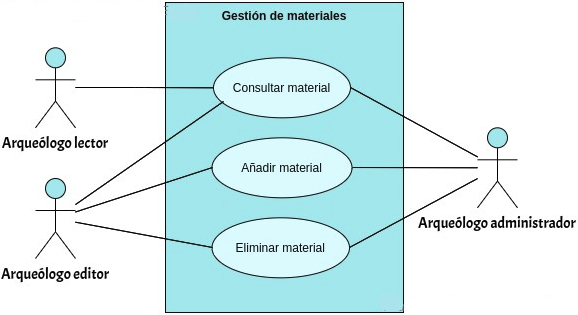
\includegraphics[scale=0.60]{imagenes/diagramas CU/material-UC.png}
        \caption{Gestión de materiales}
        \label{fig:material-management}
    \end{figure}

\subsubsection{Caso de uso 6.1: Consultar material}

    \begin{table}[H]
    \begin{center}
        \begin{adjustbox}{width=\textwidth}
        \begin{tabular}{ | l | l | l | l | c | c | } 
            \hline
            \textbf{Caso de uso} & \multicolumn{4}{l|}{Consultar material} & \cellcolor{gray!50} \textbf{CU-6.1}\\
            \hline
            \textbf{Actores} & \multicolumn{5}{p{0.9\linewidth}|}{Arqueólogo lector, arqueólogo editor, arqueólogo administrador} \\
            \hline
            \textbf{Tipo} & \multicolumn{5}{l|}{Primario y esencial} \\
            \hline
            \textbf{Referencias} & \multicolumn{3}{l|}{RF-6.1} & \multicolumn{2}{l|}{ }\\
            \hline
            \textbf{Precondición} & \multicolumn{5}{l|}{El usuario deberá estar registrado y activo en el sistema} \\
            \hline
            \textbf{Postcondición} & \multicolumn{5}{l|}{} \\
            \hline
            \textbf{Autor} & \multicolumn{1}{p{0.25\linewidth}|}{Joaquín Alejandro España Sánchez} & \textbf{Fecha} & 
            17-02-2022     & \textbf{Versión}                                                      & 1.0\\
            \hline
        \end{tabular}
        \end{adjustbox}
        \caption{CU-6.1: Consultar material}
        \label{tab:consult-material}
    \end{center}
    \end{table}

    \begin{table}[H]
        \centering
        \begin{tabularx}{\textwidth}{@{} |L |@{}} \hline
            \rowcolor{gray!50} 
            \textbf{Propósito} \\
            \hline
            Permite al usuario visualizar el estado actual de un material. \\
            \hline
        \end{tabularx}
    \end{table}

    \begin{table}[H]
        \centering
        \begin{tabularx}{\textwidth}{@{} |L |@{}} \hline
            \rowcolor{gray!50} 
            \textbf{Resumen} \\
            \hline
            Permite a un determinado tipo de arqueólogo con permisos ver los datos asociados
            a un material. \\
            \hline
        \end{tabularx}
    \end{table}

\subsubsection{Caso de uso 6.2: Añadir material}

    \begin{table}[H]
        \begin{center}
            \begin{adjustbox}{width=\textwidth}
            \begin{tabular}{ | l | l | l | l | c | c | } 
                \hline
                \textbf{Caso de uso} & \multicolumn{4}{l|}{Añadir material} & \cellcolor{gray!50} \textbf{CU-6.2}\\
                \hline
                \textbf{Actores} & \multicolumn{5}{p{0.9\linewidth}|}{Arqueólogo editor, arqueólogo administrador} \\
                \hline
                \textbf{Tipo} & \multicolumn{5}{l|}{Primario y esencial} \\
                \hline
                \textbf{Referencias} & \multicolumn{3}{l|}{RF-6.2} & \multicolumn{2}{l|}{ }\\
                \hline
                \textbf{Precondición} & \multicolumn{5}{l|}{El usuario deberá estar registrado y activo en el sistema} \\
                \hline
                \textbf{Postcondición} & \multicolumn{5}{l|}{El usuario debe haber podido añadir un material nuevo} \\
                \hline
                \textbf{Autor} & \multicolumn{1}{p{0.25\linewidth}|}{Joaquín Alejandro España Sánchez} & \textbf{Fecha} & 
                17-02-2022     & \textbf{Versión}                                                      & 1.0\\
                \hline
            \end{tabular}
            \end{adjustbox}
            \caption{CU-6.2: Añadir material}
            \label{tab:add-material}
        \end{center}
        \end{table}

        \begin{table}[H]
            \centering
            \begin{tabularx}{\textwidth}{@{} |L |@{}} \hline
                \rowcolor{gray!50} 
                \textbf{Propósito} \\
                \hline
                Permite a un usuario añadir un nuevo material al sistema. \\
                \hline
            \end{tabularx}
        \end{table}
    
        \begin{table}[H]
            \centering
            \begin{tabularx}{\textwidth}{@{} |L |@{}} \hline
                \rowcolor{gray!50} 
                \textbf{Resumen} \\
                \hline
                Permite almacenar un nuevo material en el sistema tras introducir los datos
                necesarios del material en el formulario correspondiente.\\
                \hline
            \end{tabularx}
        \end{table}


\subsubsection{Caso de uso 6.3: Eliminar material}

    \begin{table}[H]
    \begin{center}
        \begin{adjustbox}{width=\textwidth}
        \begin{tabular}{ | l | l | l | l | c | c | } 
            \hline
            \textbf{Caso de uso} & \multicolumn{4}{l|}{Eliminar material} & \cellcolor{gray!50} \textbf{CU-6.3}\\
            \hline
            \textbf{Actores} & \multicolumn{5}{p{0.9\linewidth}|}{Arqueólogo editor, arqueólogo administrador} \\
            \hline
            \textbf{Tipo} & \multicolumn{5}{l|}{Primario y esencial} \\
            \hline
            \textbf{Referencias} & \multicolumn{3}{l|}{RF-6.3} & \multicolumn{2}{l|}{ }\\
            \hline
            \textbf{Precondición} & \multicolumn{5}{l|}{El usuario deberá estar registrado y activo en el sistema} \\
            \hline
            \textbf{Postcondición} & \multicolumn{5}{l|}{El material y toda la información asociada se eliminarán del sistema} \\
            \hline
            \textbf{Autor} & \multicolumn{1}{p{0.25\linewidth}|}{Joaquín Alejandro España Sánchez} & \textbf{Fecha} & 
            17-02-2022     & \textbf{Versión}                                                      & 1.0\\
            \hline
        \end{tabular}
        \end{adjustbox}
        \caption{CU-6.3: Eliminar material}
        \label{tab:delete-material}
    \end{center}
    \end{table}

    \begin{table}[H]
        \centering
        \begin{tabularx}{\textwidth}{@{} |L |@{}} \hline
            \rowcolor{gray!50} 
            \textbf{Propósito} \\
            \hline
            Permite a un usuario eliminar cualquier información asociada a un material. \\
            \hline
        \end{tabularx}
    \end{table}

    \begin{table}[H]
        \centering
        \begin{tabularx}{\textwidth}{@{} |L |@{}} \hline
            \rowcolor{gray!50} 
            \textbf{Resumen} \\
            \hline
            El arqueólogo editor o administrador con permisos podrá eliminar un determinado
            material previamente almacenado en el sistema. \\
            \hline
        \end{tabularx}
    \end{table}

\subsection{Gestión de usuarios}
    \begin{figure}[H]
        \centering
        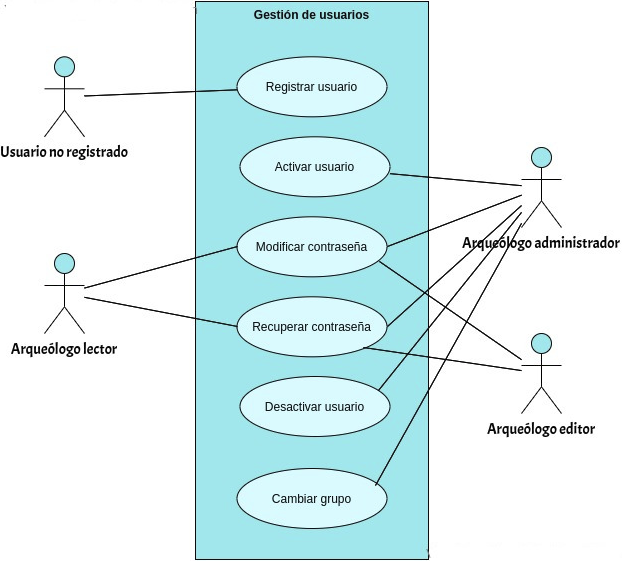
\includegraphics[scale=0.50]{imagenes/diagramas CU/user-UC.png}
        \caption{Gestión de usuarios}
        \label{fig:user-management}
    \end{figure}

\subsubsection{Caso de uso 7.1: Registrar usuario}

    \begin{table}[H]
    \begin{center}
        \begin{adjustbox}{width=\textwidth}
        \begin{tabular}{ | l | l | l | l | c | c | } 
            \hline
            \textbf{Caso de uso} & \multicolumn{4}{l|}{Registrar usuario} & \cellcolor{gray!50} \textbf{CU-7.1}\\
            \hline
            \textbf{Actores} & \multicolumn{5}{p{0.9\linewidth}|}{Usuario no registrado} \\
            \hline
            \textbf{Tipo} & \multicolumn{5}{l|}{Primario y esencial} \\
            \hline
            \textbf{Referencias} & \multicolumn{3}{l|}{RF-7.1} & \multicolumn{2}{l|}{ }\\
            \hline
            \textbf{Precondición} & \multicolumn{5}{l|}{ } \\
            \hline
            \textbf{Postcondición} & \multicolumn{5}{l|}{El usuario habrá enviado la petición de registro correctamente en el
            sistema} \\
            \hline
            \textbf{Autor} & \multicolumn{1}{p{0.25\linewidth}|}{Joaquín Alejandro España Sánchez} & \textbf{Fecha} & 
            17-02-2022     & \textbf{Versión}                                                      & 1.0\\
            \hline
        \end{tabular}
        \end{adjustbox}
        \caption{CU-7.1: Registrar usuario}
        \label{tab:register-user}
    \end{center}
    \end{table}

    \begin{table}[H]
        \centering
        \begin{tabularx}{\textwidth}{@{} |L |@{}} \hline
            \rowcolor{gray!50} 
            \textbf{Propósito} \\
            \hline
            Permitir a usuarios no registrados en el sistema enviar una petición de registro. \\
            \hline
        \end{tabularx}
    \end{table}

    \begin{table}[H]
        \centering
        \begin{tabularx}{\textwidth}{@{} |L |@{}} \hline
            \rowcolor{gray!50} 
            \textbf{Resumen} \\
            \hline
            Un usuario no registrado en el sistema accederá a la página web del sitio y tras
            rellenar un formulario podrá enviar una solicitud de registro en el sistema. \\
            \hline
        \end{tabularx}
    \end{table}


\subsubsection{Caso de uso 7.2: Activar usuario}

    \begin{table}[H]
    \begin{center}
        \begin{adjustbox}{width=\textwidth}
        \begin{tabular}{ | l | l | l | l | c | c | } 
            \hline
            \textbf{Caso de uso} & \multicolumn{4}{l|}{Activar usuario} & \cellcolor{gray!50} \textbf{CU-7.2}\\
            \hline
            \textbf{Actores} & \multicolumn{5}{p{0.9\linewidth}|}{Arqueólogo administrador} \\
            \hline
            \textbf{Tipo} & \multicolumn{5}{l|}{Primario y esencial} \\
            \hline
            \textbf{Referencias} & \multicolumn{3}{l|}{RF-7.2} & \multicolumn{2}{l|}{ }\\
            \hline
            \textbf{Precondición} & \multicolumn{5}{l|}{Deberá existir una petición de registro previa} \\
            \hline
            \textbf{Postcondición} & \multicolumn{5}{l|}{El usuario solicitante habrá sido activado en el sistema} \\
            \hline
            \textbf{Autor} & \multicolumn{1}{p{0.25\linewidth}|}{Joaquín Alejandro España Sánchez} & \textbf{Fecha} & 
            17-02-2022     & \textbf{Versión}                                                      & 1.0\\
            \hline
        \end{tabular}
        \end{adjustbox}
        \caption{CU-7.2: Activar usuario}
        \label{tab:activate-user}
    \end{center}
    \end{table}

    \begin{table}[H]
        \centering
        \begin{tabularx}{\textwidth}{@{} |L |@{}} \hline
            \rowcolor{gray!50} 
            \textbf{Propósito} \\
            \hline
            Permite a un arqueólogo administrador activar a un usuario. \\
            \hline
        \end{tabularx}
    \end{table}

    \begin{table}[H]
        \centering
        \begin{tabularx}{\textwidth}{@{} |L |@{}} \hline
            \rowcolor{gray!50} 
            \textbf{Resumen} \\
            \hline
            El arqueólogo administrador, tras haber recibido una solicitud de registro por parte
            de un usuario no registrado, podrá activarlo en el sistema. \\
            \hline
        \end{tabularx}
    \end{table}

\subsubsection{Caso de uso 7.3: Modificar contraseña}

    \begin{table}[H]
    \begin{center}
        \begin{adjustbox}{width=\textwidth}
        \begin{tabular}{ | l | l | l | l | c | c | } 
            \hline
            \textbf{Caso de uso} & \multicolumn{4}{l|}{Modificar contraseña} & \cellcolor{gray!50} \textbf{CU-7.3}\\
            \hline
            \textbf{Actores} & \multicolumn{5}{p{0.9\linewidth}|}{Arqueólogo administrador} \\
            \hline
            \textbf{Tipo} & \multicolumn{5}{l|}{Primario y esencial} \\
            \hline
            \textbf{Referencias} & \multicolumn{3}{l|}{RF-7.3} & \multicolumn{2}{l|}{ }\\
            \hline
            \textbf{Precondición} & \multicolumn{5}{l|}{El usuario deberá estar registrado y activo en el sistema} \\
            \hline
            \textbf{Postcondición} & \multicolumn{5}{l|}{La contraseña del usuario habrá modificado su valor anterior} \\
            \hline
            \textbf{Autor} & \multicolumn{1}{p{0.25\linewidth}|}{Joaquín Alejandro España Sánchez} & \textbf{Fecha} & 
            17-02-2022     & \textbf{Versión}                                                      & 1.0\\
            \hline
        \end{tabular}
        \end{adjustbox}
        \caption{CU-7.3: Modificar contraseña}
        \label{tab:modify-password}
    \end{center}
    \end{table}

    \begin{table}[H]
        \centering
        \begin{tabularx}{\textwidth}{@{} |L |@{}} \hline
            \rowcolor{gray!50} 
            \textbf{Propósito} \\
            \hline
            Permite a un usuario registrado y activo en el sistema cambiar su contraseña. \\
            \hline
        \end{tabularx}
    \end{table}

    \begin{table}[H]
        \centering
        \begin{tabularx}{\textwidth}{@{} |L |@{}} \hline
            \rowcolor{gray!50} 
            \textbf{Resumen} \\
            \hline
            El usuario podrá cambiar su antigua contraseña previamente almacenada directamente
            desde el sitio web.\\
            \hline
        \end{tabularx}
    \end{table}

\subsubsection{Caso de uso 7.4: Recuperar contraseña}

    \begin{table}[H]
    \begin{center}
        \begin{adjustbox}{width=\textwidth}
        \begin{tabular}{ | l | l | l | l | c | c | } 
            \hline
            \textbf{Caso de uso} & \multicolumn{4}{l|}{Recuperar contraseña} & \cellcolor{gray!50} \textbf{CU-7.4}\\
            \hline
            \textbf{Actores} & \multicolumn{5}{p{0.9\linewidth}|}{Arqueólogo lector, arqueólogo editor, arqueólogo administrador} \\
            \hline
            \textbf{Tipo} & \multicolumn{5}{l|}{Primario y esencial} \\
            \hline
            \textbf{Referencias} & \multicolumn{3}{l|}{RF-7.4} & \multicolumn{2}{l|}{ }\\
            \hline
            \textbf{Precondición} & \multicolumn{5}{l|}{El usuario deberá estar registrado y activo en el sistema} \\
            \hline
            \textbf{Postcondición} & \multicolumn{5}{l|}{El usuario habrá podido restablecer su contraseña} \\
            \hline
            \textbf{Autor} & \multicolumn{1}{p{0.25\linewidth}|}{Joaquín Alejandro España Sánchez} & \textbf{Fecha} & 
            17-02-2022     & \textbf{Versión}                                                      & 1.0\\
            \hline
        \end{tabular}
        \end{adjustbox}
        \caption{CU-7.4: Recuperar contraseña}
        \label{tab:reset-password}
    \end{center}
    \end{table}

    \begin{table}[H]
        \centering
        \begin{tabularx}{\textwidth}{@{} |L |@{}} \hline
            \rowcolor{gray!50} 
            \textbf{Propósito} \\
            \hline
            Permite a un usuario ya registrado en el sistema cambiar su contraseña en caso
            de olvido. \\
            \hline
        \end{tabularx}
    \end{table}

    \begin{table}[H]
        \centering
        \begin{tabularx}{\textwidth}{@{} |L |@{}} \hline
            \rowcolor{gray!50} 
            \textbf{Resumen} \\
            \hline
            El usuario previamente registrado en el sistema podrá restablecer su contraseña sin
            entrar en el sitio web por medio de un formulario en el que debe introducir el correo
            electrónico con el que se registró. \\
            \hline
        \end{tabularx}
    \end{table}

\subsubsection{Caso de uso 7.5: Desactivar usuario}

    \begin{table}[H]
    \begin{center}
        \begin{adjustbox}{width=\textwidth}
        \begin{tabular}{ | l | l | l | l | c | c | } 
            \hline
            \textbf{Caso de uso} & \multicolumn{4}{l|}{Desactivar usuario} & \cellcolor{gray!50} \textbf{CU-7.5}\\
            \hline
            \textbf{Actores} & \multicolumn{5}{p{0.9\linewidth}|}{Arqueólogo administrador} \\
            \hline
            \textbf{Tipo} & \multicolumn{5}{l|}{Primario y esencial} \\
            \hline
            \textbf{Referencias} & \multicolumn{3}{l|}{RF-7.5} & \multicolumn{2}{l|}{ }\\
            \hline
            \textbf{Precondición} & \multicolumn{5}{l|}{El usuario deberá estar activo en el sistema} \\
            \hline
            \textbf{Postcondición} & \multicolumn{5}{l|}{El usuario habrá quedado inactivo en el sistema} \\
            \hline
            \textbf{Autor} & \multicolumn{1}{p{0.25\linewidth}|}{Joaquín Alejandro España Sánchez} & \textbf{Fecha} & 
            17-02-2022     & \textbf{Versión}                                                      & 1.0\\
            \hline
        \end{tabular}
        \end{adjustbox}
        \caption{CU-7.5: Desactivar usuario}
        \label{tab:deactivate-user}
    \end{center}
    \end{table}

    \begin{table}[H]
        \centering
        \begin{tabularx}{\textwidth}{@{} |L |@{}} \hline
            \rowcolor{gray!50} 
            \textbf{Propósito} \\
            \hline
            Permite a un arqueólogo administrador desactivar a un usuario. \\
            \hline
        \end{tabularx}
    \end{table}

    \begin{table}[H]
        \centering
        \begin{tabularx}{\textwidth}{@{} |L |@{}} \hline
            \rowcolor{gray!50} 
            \textbf{Resumen} \\
            \hline
            El arqueólogo administrador podrá desactivar a un usuario previamente activo en el
            sistema. \\
            \hline
        \end{tabularx}
    \end{table}


\subsubsection{Caso de uso 7.6: Cambiar grupo}

\begin{table}[H]
    \begin{center}
        \begin{adjustbox}{width=\textwidth}
        \begin{tabular}{ | l | l | l | l | c | c | } 
            \hline
            \textbf{Caso de uso} & \multicolumn{4}{l|}{Cambiar grupo} & \cellcolor{gray!50} \textbf{CU-7.6}\\
            \hline
            \textbf{Actores} & \multicolumn{5}{p{0.9\linewidth}|}{Arqueólogo administrador} \\
            \hline
            \textbf{Tipo} & \multicolumn{5}{l|}{Primario y esencial} \\
            \hline
            \textbf{Referencias} & \multicolumn{3}{l|}{RF-7.6} & \multicolumn{2}{l|}{ }\\
            \hline
            \textbf{Precondición} & \multicolumn{5}{l|}{El usuario deberá estar registrado en el sistema} \\
            \hline
            \textbf{Postcondición} & \multicolumn{5}{l|}{Se habrá modificado el grupo al que pertenece el usuario correctamente} \\
            \hline
            \textbf{Autor} & \multicolumn{1}{p{0.25\linewidth}|}{Joaquín Alejandro España Sánchez} & \textbf{Fecha} & 
            17-02-2022     & \textbf{Versión}                                                      & 1.0\\
            \hline
        \end{tabular}
        \end{adjustbox}
        \caption{CU-7.6: Cambiar grupo}
        \label{tab:change-group}
    \end{center}
    \end{table}

    \begin{table}[H]
        \centering
        \begin{tabularx}{\textwidth}{@{} |L |@{}} \hline
            \rowcolor{gray!50} 
            \textbf{Propósito} \\
            \hline
            Permite a un arqueólogo administrador cambiar de grupo de permisos a un usuario
            registrado en el sistema. \\
            \hline
        \end{tabularx}
    \end{table}

    \begin{table}[H]
        \centering
        \begin{tabularx}{\textwidth}{@{} |L |@{}} \hline
            \rowcolor{gray!50} 
            \textbf{Resumen} \\
            \hline
            El arqueólogo administrador podrá cambiar de grupo de permisos a un usuario que esté
            registrado en el sistema a través de un panel de administración al que solo él tendrá
            acceso. \\
            \hline
        \end{tabularx}
    \end{table}

Como hemos mencionado en el apartado \ref{sec:actors}, se ha obviado el administrador del
sistema en los diagramas de Casos de Uso para una mayor comprensión y claridad.
